\documentclass[aspectratio=169,11pt]{beamer}

\usetheme{default}
\usecolortheme{dove}
\setbeamertemplate{navigation symbols}{}
\setbeamertemplate{footline}[frame number]
\setbeamertemplate{frametitle}{\vspace{0.3cm}\insertframetitle}

\usepackage[T1]{fontenc}
% \usepackage{lmodern}
\usepackage{amsmath,amssymb}
\usepackage{mathtools}
\usepackage{tikz}
\usetikzlibrary{positioning,arrows.meta,calc,fit,decorations.pathreplacing,backgrounds}
\usepackage{xcolor}
\usepackage{array}
\usepackage{booktabs}

\renewcommand{\leq}{\leqslant}
\renewcommand{\geq}{\geqslant}
\newcommand{\Oh}{\mathcal{O}}
\newcommand{\strips}{\mathtt{strips}}

\definecolor{nczone}{RGB}{200,210,240}
\definecolor{darkblue}{RGB}{40,60,120}
\definecolor{darkred}{RGB}{150,30,30}
\definecolor{slab1}{RGB}{230,180,180}
\definecolor{slab2}{RGB}{180,200,230}
\definecolor{slab3}{RGB}{200,230,180}
\definecolor{slab4}{RGB}{245,225,160}
\definecolor{slab5}{RGB}{210,195,230}

\setbeamercolor{block title}{bg=darkblue!15,fg=darkblue}
\setbeamercolor{block body}{bg=darkblue!5}
\setbeamercolor{block title alerted}{bg=darkred!15,fg=darkred}
\setbeamercolor{block body alerted}{bg=darkred!5}

\title{Dynamic data structures for twin-ordered matrices}
\subtitle{Queries and updates in $\Oh(\log\log n)$ expected worst-case time}
\author{B.~Bosek \and J.~Czy\.{z}ewska \and E.~Kipouridis \and W.~Nadara \and M.~Pilipczuk \and K.~W\k{e}grzycki \and A.~Zych-Pawlewicz}
\institute{Jagiellonian University \quad University of Warsaw \quad MPI for Informatics}
\date{LATIN 2026}

\begin{document}

%% ============== SLIDE 1: Title ==============
\begin{frame}
\titlepage
\end{frame}

%% ============== SLIDE 2: Object ==============
\begin{frame}{What is the object we want to maintain?}
\begin{columns}[T]
\begin{column}{0.52\textwidth}
\vspace{0.3cm}
{\Large $M \in \{0,1\}^{n\times n}$}
\medskip
\begin{itemize}
\item Rows and columns stay in a fixed order
\item The matrix is always promised to be $d$-twin-ordered
\item We need cell queries and single-cell flips
\end{itemize}
\smallskip
{\small\color{gray} The order is fixed throughout the paper.}
\end{column}
\begin{column}{0.44\textwidth}
\centering
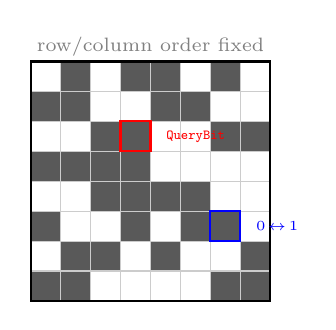
\begin{tikzpicture}[scale=0.38]
\foreach \r/\data [count=\ri from 0] in {
  0/{0,1,0,1,1,0,1,0},
  1/{1,1,0,0,1,1,0,0},
  2/{0,0,1,1,0,0,1,1},
  3/{1,1,1,1,0,0,0,0},
  4/{0,0,1,1,1,1,0,0},
  5/{1,0,0,1,0,1,1,0},
  6/{0,1,1,0,1,0,0,1},
  7/{1,1,0,0,0,0,1,1}}{
  \foreach \v [count=\ci from 0] in \data {
    \ifnum\v=1 \fill[black!65] (\ci,7-\ri) rectangle ++(1,1);
    \else \fill[white] (\ci,7-\ri) rectangle ++(1,1);
    \fi
  }
}
\draw[step=1,gray!40,thin] (0,0) grid (8,8);
\draw[thick] (0,0) rectangle (8,8);
\draw[red,thick] (3,5) rectangle (4,6);
\node[red,font=\tiny,anchor=west] at (4.2,5.5) {\texttt{QueryBit}};
\draw[blue,thick] (6,2) rectangle (7,3);
\node[blue,font=\tiny,anchor=west] at (7.2,2.5) {$0\!\leftrightarrow\!1$};
\node[font=\scriptsize,gray] at (4,8.5) {row/column order fixed};
\end{tikzpicture}

\bigskip
{\large\texttt{QueryBit}$(i,j)$}\\[4pt]
{\large\texttt{Update}$(i,j)$}
\end{column}
\end{columns}
\end{frame}

%% ============== SLIDE 3: Twin-ordering ==============
\begin{frame}{Twin-ordering by contraction sequences}
\begin{itemize}
\item A \emph{contraction sequence}: $(\mathcal{R}_0,\mathcal{C}_0),\ldots,(\mathcal{R}_p,\mathcal{C}_p)$
\item Starts with singleton blocks $\to$ ends with one row block and one column block
\item Each step: merge two consecutive row blocks or two consecutive column blocks
\item Width $\leq d$: at every step, every row/column block has $\leq d$ non-constant zones
\end{itemize}

\medskip
\begin{alertblock}{}
$M$ is $d$-\emph{twin-ordered} iff it admits such a contraction sequence.
\end{alertblock}

\medskip
\centering
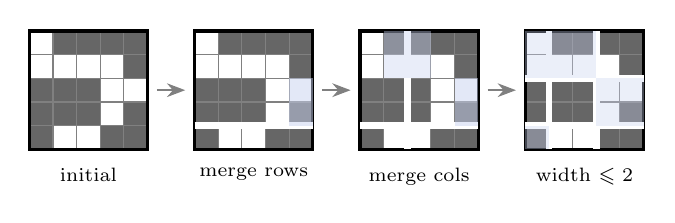
\begin{tikzpicture}[scale=0.30]
% Helper for drawing a 5x5 matrix
% State 1
\begin{scope}
\foreach \r/\d [count=\ri from 0] in {
0/{0,1,1,1,1},1/{0,0,0,0,1},2/{1,1,1,0,0},3/{1,1,1,0,1},4/{1,0,0,1,1}}{
\foreach \v [count=\ci from 0] in \d {
\ifnum\v=1 \fill[black!60] (\ci,4-\ri) rectangle ++(1,1);
\else \fill[white] (\ci,4-\ri) rectangle ++(1,1); \fi}}
\draw[step=1,gray] (0,0) grid (5,5);
\draw[very thick] (0,0) rectangle (5,5);
\node[below,font=\scriptsize] at (2.5,-0.4) {initial};
\end{scope}
\draw[-{Stealth},thick,gray] (5.4,2.5)--(6.6,2.5);
% State 2: merge rows 3,4
\begin{scope}[shift={(7,0)}]
\foreach \r/\d [count=\ri from 0] in {
0/{0,1,1,1,1},1/{0,0,0,0,1},2/{1,1,1,0,0},3/{1,1,1,0,1},4/{1,0,0,1,1}}{
\foreach \v [count=\ci from 0] in \d {
\ifnum\v=1 \fill[black!60] (\ci,4-\ri) rectangle ++(1,1);
\else \fill[white] (\ci,4-\ri) rectangle ++(1,1); \fi}}
\draw[step=1,gray] (0,0) grid (5,5);
\draw[very thick] (0,0) rectangle (5,5);
\draw[white,line width=2.5pt] (0,1)--(5,1);
\fill[nczone,opacity=0.5] (4,1) rectangle (5,3);
\node[below,font=\scriptsize] at (2.5,-0.4) {merge rows};
\end{scope}
\draw[-{Stealth},thick,gray] (12.4,2.5)--(13.6,2.5);
% State 3: also merge cols 2,3
\begin{scope}[shift={(14,0)}]
\foreach \r/\d [count=\ri from 0] in {
0/{0,1,1,1,1},1/{0,0,0,0,1},2/{1,1,1,0,0},3/{1,1,1,0,1},4/{1,0,0,1,1}}{
\foreach \v [count=\ci from 0] in \d {
\ifnum\v=1 \fill[black!60] (\ci,4-\ri) rectangle ++(1,1);
\else \fill[white] (\ci,4-\ri) rectangle ++(1,1); \fi}}
\draw[step=1,gray] (0,0) grid (5,5);
\draw[very thick] (0,0) rectangle (5,5);
\draw[white,line width=2.5pt] (0,1)--(5,1);
\draw[white,line width=2.5pt] (2,0)--(2,5);
\fill[nczone,opacity=0.5] (4,1) rectangle (5,3);
\fill[nczone,opacity=0.4] (1,3) rectangle (3,5);
\node[below,font=\scriptsize] at (2.5,-0.4) {merge cols};
\end{scope}
\draw[-{Stealth},thick,gray] (19.4,2.5)--(20.6,2.5);
% State 4: late
\begin{scope}[shift={(21,0)}]
\foreach \r/\d [count=\ri from 0] in {
0/{0,1,1,1,1},1/{0,0,0,0,1},2/{1,1,1,0,0},3/{1,1,1,0,1},4/{1,0,0,1,1}}{
\foreach \v [count=\ci from 0] in \d {
\ifnum\v=1 \fill[black!60] (\ci,4-\ri) rectangle ++(1,1);
\else \fill[white] (\ci,4-\ri) rectangle ++(1,1); \fi}}
\draw[step=1,gray] (0,0) grid (5,5);
\draw[very thick] (0,0) rectangle (5,5);
\draw[white,line width=2.5pt] (0,1)--(5,1);
\draw[white,line width=2.5pt] (0,3)--(5,3);
\draw[white,line width=2.5pt] (1,0)--(1,5);
\draw[white,line width=2.5pt] (3,0)--(3,5);
\fill[nczone,opacity=0.35] (0,3) rectangle (1,5);
\fill[nczone,opacity=0.35] (1,3) rectangle (3,5);
\fill[nczone,opacity=0.35] (3,1) rectangle (5,3);
\fill[nczone,opacity=0.35] (0,0) rectangle (1,1);
\node[below,font=\scriptsize] at (2.5,-0.4) {width $\leq 2$};
\end{scope}
\end{tikzpicture}
\end{frame}

%% ============== SLIDE 4: The gap ==============
\begin{frame}{The gap: static yes, dynamic no}
\begin{columns}[T]
\begin{column}{0.46\textwidth}
\begin{block}{Static compact repr.\ {\small[PSZ, STACS'22]}}
\begin{itemize}
\item $\Oh_d(n)$ bits of space
\item Queries in $\Oh_d(\log\log n)$
\item Fundamentally static
\end{itemize}
\end{block}
\end{column}
\begin{column}{0.46\textwidth}
\begin{alertblock}{Our dynamic question}
\begin{itemize}
\item Support \texttt{QueryBit} and \texttt{Update}
\item $M$ stays $d$-twin-ordered at every moment
\item Near-linear memory on word RAM?
\end{itemize}
\end{alertblock}
\end{column}
\end{columns}

\bigskip
\centering
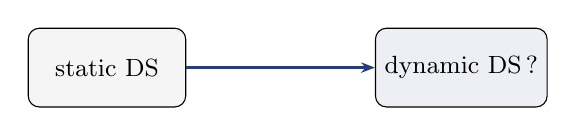
\begin{tikzpicture}
\node[draw,rounded corners,minimum width=2cm,minimum height=1cm,fill=gray!8] (s) at (0,0) {\small static DS};
\node[draw,rounded corners,minimum width=2cm,minimum height=1cm,fill=darkblue!8] (d) at (4.5,0) {\small dynamic DS\,?};
\draw[-{Stealth[length=5pt]},very thick,darkblue] (s)--(d);
\end{tikzpicture}

\smallskip
{\small This is exactly the problem addressed by Theorem~1 of the paper.}
\end{frame}

%% ============== SLIDE 5: Main theorem ==============
\begin{frame}{Main theorem}
\begin{block}{\textbf{Theorem 1.}}
Let $d\in\mathbb{N}$ and $M\in\{0,1\}^{n\times n}$ be updated over time, always remaining $d$-twin-ordered.
There exists a dynamic data structure using $\Oh_d(n)$ memory supporting:
\begin{itemize}
\item $\mathtt{Init}(n,\mathcal{K})$ \hfill $\Oh_d\!\bigl((n+|\mathcal{K}|)\log\log n\bigr)$
\item $\mathtt{QueryBit}(i,j)$ \hfill $\Oh(\log\log n)$ expected worst-case
\item $\mathtt{Update}(i,j)$ \hfill $\Oh(\log\log n)$ expected worst-case
\end{itemize}
\end{block}

\smallskip
{\small $\mathcal{K}$: list of disjoint rectangles covering all ones. \quad Word RAM model: $\Oh_d(n)$ memory $=\Oh_d(n\log n)$ bits.}

\medskip
{\small Only initialization time and memory depend on $d$.}

\bigskip
\centering
\begin{tabular}{lccc}
\toprule
& \textbf{Space} & \textbf{Query} & \textbf{Update}\\
\midrule
Static [PSZ'22] & $\Oh_d(n)$ bits & $\Oh_d(\log\log n)$ & ---\\
\textbf{Dynamic [this work]} & $\Oh_d(n)$ memory & $\Oh(\log\log n)$ & $\Oh(\log\log n)$\\
\bottomrule
\end{tabular}
\end{frame}

%% ============== SLIDE 6: Slabs ==============
\begin{frame}{Slabs: why near-linear space is possible}
A \emph{slab} is a zone $M\bigl[[a,b],[c,d]\bigr]$ entirely filled with ones.

A \emph{slab decomposition} $\mathcal{K}$: pairwise disjoint slabs covering all ones.

\medskip
\begin{alertblock}{}
$|\mathcal{K}| \leq d(2n-2)+1$
\end{alertblock}

{\small Every $d$-twin-ordered matrix admits an $\Oh_d(n)$-size rectangle description of all ones.}

\bigskip
\begin{columns}
\begin{column}{0.45\textwidth}
\centering
% Figure 2 adaptation: 5x5 matrix with colored slabs
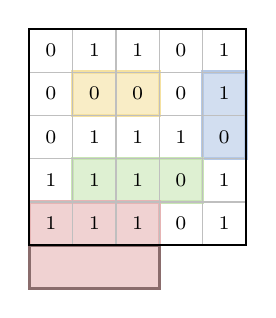
\begin{tikzpicture}[scale=0.55]
\def\M{
{0,1,1,0,1},
{0,0,0,0,1},
{0,1,1,1,0},
{1,1,1,0,1},
{1,1,1,0,1}}
% Draw slabs first
\fill[slab4,opacity=0.6] (1,3) rectangle (3,4); % [1,1],[2,3]
\fill[slab2,opacity=0.6] (4,3) rectangle (5,4); % [1,2],[5,5] row1
\fill[slab2,opacity=0.6] (4,2) rectangle (5,3); % [1,2],[5,5] row2
\fill[slab3,opacity=0.6] (1,1) rectangle (4,2); % [3,3],[2,4]
\fill[slab1,opacity=0.6] (0,0) rectangle (3,1); % [4,5],[1,3] row5
\fill[slab1,opacity=0.6] (0,-1) rectangle (3,0); % [4,5],[1,3] row4... 
% Redo properly with row 0 at top
% Let me just place values
\foreach \r [count=\ri from 0] in \M {
\foreach \v [count=\ci from 0] in \r {
\node[font=\scriptsize] at (\ci+0.5,4.5-\ri) {\v};
}}
% Slab outlines
\draw[slab4,very thick] (1,3) rectangle (3,4);
\draw[slab2,very thick] (4,2) rectangle (5,4);
\draw[slab3,very thick] (1,1) rectangle (4,2);
\draw[slab1,very thick] (0,0) rectangle (3,1);
\draw[slab1!60!black,very thick] (0,-1) rectangle (3,0);
% Hmm, indexing is tricky. Let me simplify.
\draw[step=1,gray!50] (0,0) grid (5,5);
\draw[thick] (0,0) rectangle (5,5);
\end{tikzpicture}
\end{column}
\begin{column}{0.5\textwidth}
{\small
Slab decomposition of the example:\\[4pt]
$M\bigl[[1,1],[2,3]\bigr]$\\
$M\bigl[[1,2],[5,5]\bigr]$\\
$M\bigl[[3,3],[2,4]\bigr]$\\
$M\bigl[[4,5],[1,3]\bigr]$, \;$M\bigl[[4,5],[5,5]\bigr]$

\medskip
Each slab stored as four coordinates $(a,b,c,d)$.
}
\end{column}
\end{columns}
\end{frame}

%% ============== SLIDE 7: Canonical slabs ==============
\begin{frame}{Canonical slabs: the normalization step}
\begin{itemize}
\item An $i$-\emph{strip}: a maximal all-ones slab of width 1 in column $i$
\item $\strips_i$: the set of all $i$-strips
\item \emph{Siblings}: strips with the same row interval persisting through consecutive columns
\end{itemize}

\begin{alertblock}{}
A \emph{canonical slab} is the union of one sibling class; each strip belongs to exactly one canonical slab.
\end{alertblock}

\[
|\mathcal{R}| \leq 4f_d(n+2)+4n \in \Oh_d(n)
\]
{\small Canonical slabs are still only $\Oh_d(n)$. \quad ($f_d$: constant from the corner bound.)}

\bigskip
\centering
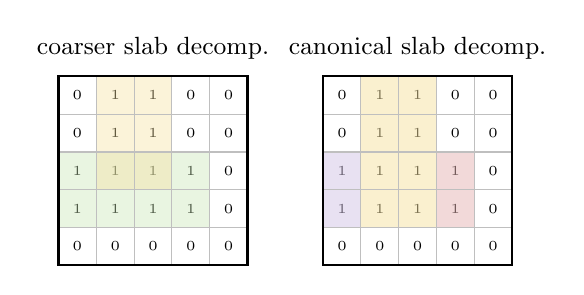
\begin{tikzpicture}[scale=0.48]
% Left: coarser decomposition (Figure 3 right matrix)
\begin{scope}
\node[above,font=\small] at (2.5,5.2) {coarser slab decomp.};
\foreach \r/\d [count=\ri from 0] in {
0/{0,1,1,0,0},1/{0,1,1,0,0},2/{1,1,1,1,0},3/{1,1,1,1,0},4/{0,0,0,0,0}}{
\foreach \v [count=\ci from 0] in \d {
\node[font=\tiny] at (\ci+0.5,4.5-\ri) {\v};
}}
\fill[slab3,opacity=0.4] (0,1) rectangle (4,3);
\fill[slab4,opacity=0.4] (1,2) rectangle (3,5);
\draw[step=1,gray!50] (0,0) grid (5,5);
\draw[thick] (0,0) rectangle (5,5);
\end{scope}
% Right: canonical
\begin{scope}[shift={(7,0)}]
\node[above,font=\small] at (2.5,5.2) {canonical slab decomp.};
\foreach \r/\d [count=\ri from 0] in {
0/{0,1,1,0,0},1/{0,1,1,0,0},2/{1,1,1,1,0},3/{1,1,1,1,0},4/{0,0,0,0,0}}{
\foreach \v [count=\ci from 0] in \d {
\node[font=\tiny] at (\ci+0.5,4.5-\ri) {\v};
}}
\fill[slab5,opacity=0.5] (0,1) rectangle (1,3);
\fill[slab4,opacity=0.5] (1,1) rectangle (3,5);
\fill[slab1,opacity=0.5] (3,1) rectangle (4,3);
\draw[step=1,gray!50] (0,0) grid (5,5);
\draw[thick] (0,0) rectangle (5,5);
\end{scope}
\end{tikzpicture}
\end{frame}

%% ============== SLIDE 8: Running example part I ==============
\begin{frame}{Running example, part I: left-to-right sweep for $B_i$}
\begin{columns}[T]
\begin{column}{0.42\textwidth}
\vspace{-0.2cm}
{\small Definitions:}
\[
O_i \coloneqq \{[a,b] \mid (a,b,i,d')\in\mathcal{K},\; d'\!\geq\! i\}
\]
\[
C_i \coloneqq \{[a,b] \mid (a,b,c',i)\in\mathcal{K},\; c'\!\leq\! i\}
\]
\[
B_i \coloneqq \strips_i \setminus \strips_{i+1}
\]

\medskip
{\small
\begin{itemize}
\item Round $i$ transforms $\strips_i$ into $\strips_{i+1}$
\item Only strips touched by slabs closing/opening matter; disappearing ones form $B_i$
\end{itemize}
}

\smallskip
{\footnotesize First half of $\mathtt{Decompose}(n,\mathcal{K})$: identify which strips disappear each round.}
\end{column}
\begin{column}{0.56\textwidth}
\centering
% Figure 4: 4x4 matrix
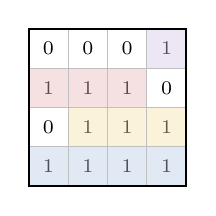
\begin{tikzpicture}[scale=0.50]
\foreach \r/\d [count=\ri from 0] in {
0/{0,0,0,1},1/{1,1,1,0},2/{0,1,1,1},3/{1,1,1,1}}{
\foreach \v [count=\ci from 0] in \d {
\node[font=\scriptsize] at (\ci+0.5,3.5-\ri) {\v};
}}
% Color the slabs: K = {(2,2,1,3),(3,3,2,4),(4,4,1,4),(1,1,4,4)}
\fill[slab1,opacity=0.4] (0,2) rectangle (3,3); % (2,2,1,3)
\fill[slab4,opacity=0.4] (1,1) rectangle (4,2); % (3,3,2,4)
\fill[slab2,opacity=0.4] (0,0) rectangle (4,1); % (4,4,1,4)
\fill[slab5,opacity=0.4] (3,3) rectangle (4,4); % (1,1,4,4)
\draw[step=1,gray!50] (0,0) grid (4,4);
\draw[thick] (0,0) rectangle (4,4);
\end{tikzpicture}

\smallskip
% Table
{\tiny
\begin{tabular}{c|c|c|c|c}
 & $O_i$ & $C_i$ & strips in $\mathbb{S}$ & $B_i$\\
\hline
$i\!=\!1$ & $\{[2,2],[4,4]\}$ & $\varnothing$ & $\{[2,2],[4,4]\}$ & $\{[2,2],[4,4]\}$\\
\hline
$i\!=\!2$ & $\{[3,3]\}$ & $\varnothing$ & $\{[2,4]\}$ & $\varnothing$\\
\hline
$i\!=\!3$ & $\varnothing$ & $\{[2,2]\}$ & $\{[2,4]\}$ & $\{[2,4]\}$\\
\hline
$i\!=\!4$ & $\{[1,1]\}$ & $\{[1,1],[3,3],[4,4]\}$ & $\{[1,1],[3,4]\}$ & $\{[1,1],[3,4]\}$\\
\end{tabular}
}
\end{column}
\end{columns}
\end{frame}

%% ============== SLIDE 9: Running example part II ==============
\begin{frame}{Running example, part II: from $A_i, B_i$ to canonical slabs}
Symmetric sweep right-to-left gives:
\[
A_i \coloneqq \strips_i \setminus \strips_{i-1}
\]

\smallskip
\begin{itemize}
\item $\mathsf{slab\_start}[a]$ remembers where the current slab on row interval $[a,b]$ started
\item When $(a,b)\in A_i$: record start $i$. \;\; When $(a,b)\in B_i$: output $(a,b,\mathsf{slab\_start}[a],i)$
\item A final left-to-right sweep over $A_i$ and $B_i$ outputs all canonical slabs
\end{itemize}

\[
\mathtt{Decompose}(n,\mathcal{K}) \text{ runs in } \Oh(n+|\mathcal{K}|\log\log n)
\]
{\small The output is the canonical slab decomposition $\mathcal{R}$.}

\bigskip
\centering
{\tiny
\begin{tabular}{c|c|c|c|c}
 & $A_i$ & $B_i$ & $\mathsf{slab\_start}_i$ & slabs added\\
\hline
$i\!=\!1$ & $\{[2,2],[4,4]\}$ & $\{[2,2],[4,4]\}$ & $[\bot,1,\bot,1]$ & $(2,2,1,1),\;(4,4,1,1)$\\
\hline
$i\!=\!2$ & $\{[2,4]\}$ & $\varnothing$ & $[\bot,2,\bot,\bot]$ & \\
\hline
$i\!=\!3$ & $\varnothing$ & $\{[2,4]\}$ & $[\bot,2,\bot,\bot]$ & $(2,4,2,3)$\\
\hline
$i\!=\!4$ & $\{[1,1],[3,4]\}$ & $\{[1,1],[3,4]\}$ & $[4,\bot,4,\bot]$ & $(1,1,4,4),\;(3,4,4,4)$\\
\end{tabular}
}

\smallskip
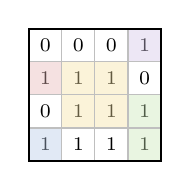
\begin{tikzpicture}[scale=0.42]
\foreach \r/\d [count=\ri from 0] in {
0/{0,0,0,1},1/{1,1,1,0},2/{0,1,1,1},3/{1,1,1,1}}{
\foreach \v [count=\ci from 0] in \d {
\node[font=\scriptsize] at (\ci+0.5,3.5-\ri) {\v};
}}
% Canonical slabs: (2,2,1,1) (4,4,1,1) (2,4,2,3) (1,1,4,4) (3,4,4,4)
\fill[slab1,opacity=0.4] (0,2) rectangle (1,3); % (2,2,1,1)
\fill[slab2,opacity=0.4] (0,0) rectangle (1,1); % (4,4,1,1)
\fill[slab4,opacity=0.4] (1,1) rectangle (3,3); % (2,4,2,3)
\fill[slab5,opacity=0.4] (3,3) rectangle (4,4); % (1,1,4,4)
\fill[slab3,opacity=0.4] (3,0) rectangle (4,2); % (3,4,4,4)
\draw[step=1,gray!50] (0,0) grid (4,4);
\draw[thick] (0,0) rectangle (4,4);
\end{tikzpicture}
\end{frame}

%% ============== SLIDE 10: Amortized structure ==============
\begin{frame}{Amortized structure: $\mathbb{P}$ for slabs, $\mathbb{Q}$ for recent flips}

{\small Take the canonical slab decomposition from slide~9 as the last rebuilt base in $\mathbb{P}$; all newer updates are kept in $\mathbb{Q}$.}

\medskip
\begin{columns}[T]
\begin{column}{0.48\textwidth}
\begin{block}{$\mathbb{P}$: static point location}
{\small Stores the canonical slab decomposition computed at last rebuild. Answers point location in $\Oh(\log\log n)$.}
\end{block}

\begin{block}{$\mathbb{Q}$: update dictionary}
{\small Hash table of explicit cell values buffered since the last rebuild.}
\end{block}
\end{column}
\begin{column}{0.48\textwidth}
{\small Buffer threshold:}
\[
|\mathbb{Q}| \leq 8f_d(n+2)
\]

{\small Invariant:}
\begin{align*}
(i,j)\in\mathbb{Q} &\Rightarrow M[i,j]=\mathbb{Q}[i,j]\\
(i,j)\notin\mathbb{Q} &\Rightarrow M[i,j]=1 \iff (i,j)\in\text{slab of }\mathbb{P}
\end{align*}
\end{column}
\end{columns}

\bigskip
\begin{itemize}
\item $\mathtt{QueryBit}(i,j)$: first check $\mathbb{Q}$; on miss, ask $\mathbb{P}$
\item $\mathtt{Update}(i,j)$: keep newest value in $\mathbb{Q}$; on first touch, recover old value from $\mathbb{P}$
\item When $|\mathbb{Q}|=8f_d(n+2)$: rebuild the base decomposition and empty the buffer
\end{itemize}

\smallskip
{\small\color{gray} Theorem~4: $\Oh(\log\log n)$ expected worst-case queries and $\Oh(\log\log n)$ expected amortized updates.}
\end{frame}

%% ============== SLIDE 11: Rebuilding ==============
\begin{frame}{Rebuilding $\mathbb{P}$: 0-updates split slabs, uncovered 1-updates become $1\!\times\!1$ slabs}

{\small Rebuilding starts from slabs in $\mathbb{P}$ and buffered values in $\mathbb{Q}$.}

\medskip
\begin{columns}[T]
\begin{column}{0.55\textwidth}
{\small Four steps:}
\begin{enumerate}
\item Partition $\mathcal{Q}$ into 0-updates and 1-updates
\item Assign 0-updates to slabs of $\mathcal{P}$ that contain them
\item Split each affected slab row-by-row; collect untouched pieces
\item Every uncovered 1-update becomes a $1\!\times\!1$ slab
\end{enumerate}

\medskip
{\small The resulting family $\mathcal{K}$ is a slab decomposition of the current matrix.}
\[
|\mathcal{K}| \leq |\mathcal{P}|+2|\mathcal{Q}|
\]
{\small Then run $\mathtt{Decompose}(n,\mathcal{K})$ to get the new canonical decomposition.}
\end{column}
\begin{column}{0.42\textwidth}
\centering
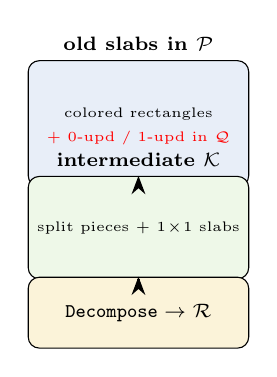
\begin{tikzpicture}[scale=0.6,font=\scriptsize]
% Old slabs panel
\node[draw,rounded corners,minimum width=2.8cm,minimum height=1.6cm,fill=slab2!30] (old) at (0,2.5) {};
\node[above,font=\scriptsize\bfseries] at (old.north) {old slabs in $\mathcal{P}$};
\node at (0,2.7) {\tiny colored rectangles};
\node[red,font=\tiny] at (0,2.2) {\tiny + 0-upd / 1-upd in $\mathcal{Q}$};

% Intermediate K
\node[draw,rounded corners,minimum width=2.8cm,minimum height=1.3cm,fill=slab3!30] (mid) at (0,0.3) {};
\node[above,font=\scriptsize\bfseries] at (mid.north) {intermediate $\mathcal{K}$};
\node[font=\tiny] at (0,0.3) {split pieces + $1\!\times\!1$ slabs};

% New canonical
\node[draw,rounded corners,minimum width=2.8cm,minimum height=0.9cm,fill=slab4!40] (fin) at (0,-1.5) {};
\node[font=\scriptsize\bfseries] at (fin) {$\mathtt{Decompose} \to \mathcal{R}$};

\draw[-{Stealth},thick] (old)--(mid);
\draw[-{Stealth},thick] (mid)--(fin);
\end{tikzpicture}

\smallskip
{\tiny\color{gray} New schematic based on Theorem~4; layout inspired by Figure~6.}
\end{column}
\end{columns}
\end{frame}

%% ============== SLIDE 12: De-amortization ==============
\begin{frame}{From amortized to worst-case: epochs and snapshot copies}

{\small Threshold: $L = 8f_d(n+2)$. \quad Partition all updates into epochs $E_0, E_1, E_2, \ldots$ of length $L$.}

\medskip
\textbf{Key idea:} one copy keeps answering updates, while the next copy is initialized in the background and then catches up.

\medskip
\begin{itemize}
\item During $E_{2i-2}$: spread $\mathtt{Init}(n,\mathcal{K})$ of the next structure over the whole epoch
\item During $E_{2i-1}$: next structure catches up (two updates per one)
\item Queries keep going to the currently active copy throughout
\end{itemize}

\medskip
{\small Two copies $\mathbb{A}_{i,0}$ (active) and $\mathbb{A}_{i,1}$ (frozen snapshot) resolve the need for uninterrupted access during initialization.}

\bigskip
\centering
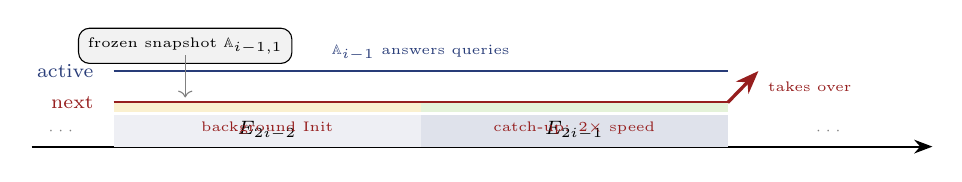
\begin{tikzpicture}[xscale=1.3,yscale=0.8,font=\small]
% Timeline
\draw[thick,-{Stealth}] (-0.3,0)--(8.5,0);
% Epochs
\fill[darkblue!8] (0.5,0) rectangle (3.5,0.5);
\fill[darkblue!15] (3.5,0) rectangle (6.5,0.5);
\node[font=\scriptsize] at (2,0.25) {$E_{2i-2}$};
\node[font=\scriptsize] at (5,0.25) {$E_{2i-1}$};
\node[font=\tiny,gray] at (0,0.25) {$\cdots$};
\node[font=\tiny,gray] at (7.5,0.25) {$\cdots$};
% Upper track: active copy
\draw[thick,darkblue] (0.5,1.2)--(6.5,1.2);
\node[font=\scriptsize,darkblue,left] at (0.4,1.2) {active};
\node[font=\tiny,above,darkblue] at (3.5,1.2) {$\mathbb{A}_{i-1}$ answers queries};
% Lower track: next copy
\draw[thick,darkred] (0.5,0.7)--(6.5,0.7);
\node[font=\scriptsize,darkred,left] at (0.4,0.7) {next};
\fill[slab4!50] (0.5,0.55) rectangle (3.5,0.7);
\node[font=\tiny] at (2,0.62) {};
\node[font=\tiny,below,darkred] at (2,0.55) {background Init};
\fill[slab3!50] (3.5,0.55) rectangle (6.5,0.7);
\node[font=\tiny,below,darkred] at (5,0.55) {catch-up: $2\times$ speed};
% Takeover
\draw[-{Stealth},very thick,darkred] (6.5,0.7)--(6.8,1.2);
\node[font=\tiny,right,darkred] at (6.8,0.95) {takes over};
% Snapshot
\node[draw,rounded corners,font=\tiny,fill=gray!10] at (1.2,1.6) {frozen snapshot $\mathbb{A}_{i-1,1}$};
\draw[->,gray,thin] (1.2,1.45)--(1.2,0.78);
\end{tikzpicture}

\smallskip
{\small\color{gray} De-amortization of Theorem~5: expected worst-case $\Oh(\log\log n)$ per update.}
\end{frame}

%% ============== SLIDE 13: Take-away ==============
\begin{frame}{Take-away}

\begin{alertblock}{}
Dynamic data structure for $d$-twin-ordered matrices:\\[2pt]
$\Oh_d(n)$ memory and $\Oh(\log\log n)$ expected worst-case time for both \texttt{QueryBit} and \texttt{Update}.
\end{alertblock}

\bigskip
\centering
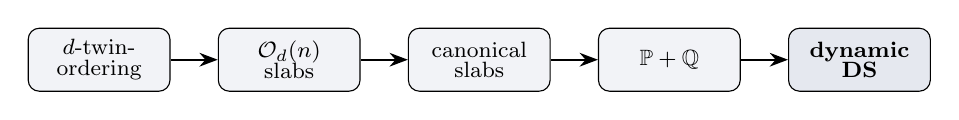
\begin{tikzpicture}[node distance=0.6cm,font=\small,
  box/.style={draw,rounded corners,minimum height=0.8cm,minimum width=1.8cm,fill=darkblue!6,align=center,font=\footnotesize}]
\node[box] (tw) {$d$-twin-\\[-2pt]ordering};
\node[box,right=of tw] (sl) {$\Oh_d(n)$\\[-2pt]slabs};
\node[box,right=of sl] (cs) {canonical\\[-2pt]slabs};
\node[box,right=of cs] (pq) {$\mathbb{P}+\mathbb{Q}$};
\node[box,right=of pq,fill=darkblue!12,font=\footnotesize\bfseries] (ds) {dynamic\\[-2pt]DS};
\draw[-{Stealth},thick] (tw)--(sl);
\draw[-{Stealth},thick] (sl)--(cs);
\draw[-{Stealth},thick] (cs)--(pq);
\draw[-{Stealth},thick] (pq)--(ds);
\end{tikzpicture}

\bigskip
{\small Structural core: canonicalization. \quad Dynamic core: buffered updates plus scheduled rebuilding.}

\vfill
\centering
{\Large\color{darkblue} Questions?}
\end{frame}

%% ============== BACKUP SLIDES ==============

\appendix

%% ============== BACKUP 14: Adhesive segment set ==============
\begin{frame}{Backup: adhesive segment set}

{\small A data structure $\mathbb{S}$ maintaining a dynamic set of pairwise disjoint, non-adjacent segments in $\{1,\ldots,n\}$.}

\medskip
Operations:
\begin{itemize}
\item $\mathtt{Containing}([a,b])$: return the segment of $S$ containing $[a,b]$
\item $\mathtt{Adjacent}([a,b])$: return segments adjacent to $[a,b]$
\item $\mathtt{Disjoint}([a,b])$: test disjointness from all segments
\item $\mathtt{Merge}([a,b])$: add $[a,b]$ and merge with adjacent segments
\item $\mathtt{Split}([a,b])$: remove $[a,b]$ from its containing segment
\end{itemize}

\medskip
{\small All operations in $\Oh(\log\log n)$ worst-case time. \quad $\Oh(n)$ memory. \quad Initialization in $\Oh(n)$.}

\bigskip
\centering
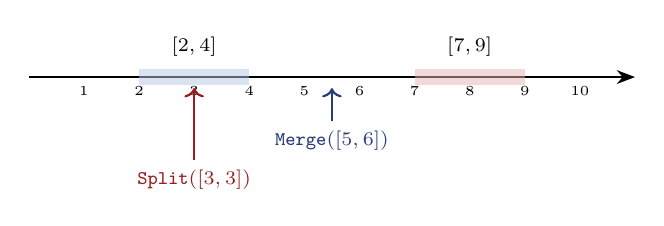
\begin{tikzpicture}[scale=0.7,font=\small]
\draw[thick,-{Stealth}] (0,0)--(11,0);
\foreach \x in {1,...,10} \node[below,font=\tiny] at (\x,0) {\x};
% Segments
\fill[slab2,opacity=0.5] (2,-0.15) rectangle (4,0.15);
\fill[slab1,opacity=0.5] (7,-0.15) rectangle (9,0.15);
\node[above,font=\scriptsize] at (3,0.2) {$[2,4]$};
\node[above,font=\scriptsize] at (8,0.2) {$[7,9]$};
% Merge example
\draw[->,thick,darkblue] (5.5,-0.8)--(5.5,-0.2);
\node[below,font=\scriptsize,darkblue] at (5.5,-0.8) {$\mathtt{Merge}([5,6])$};
% Split example
\draw[->,thick,darkred] (3,-1.5)--(3,-0.2);
\node[below,font=\scriptsize,darkred] at (3,-1.5) {$\mathtt{Split}([3,3])$};
\end{tikzpicture}
\end{frame}

%% ============== BACKUP 15: Why O_d(n) canonical slabs? ==============
\begin{frame}{Backup: why are there only $\Oh_d(n)$ canonical slabs?}

\begin{itemize}
\item A \emph{corner}: a $2\times 2$ zone whose two rows differ and two columns differ
\item \textbf{Lemma~1}: a $d$-twin-ordered matrix has $\leq f_d(n+2)$ corners, where $f_d = \tfrac{16}{3}(2d+3)^2\cdot 2^{4(2d+2)}$
\item Every ``internal'' canonical slab must intersect a corner
\item Boundary cases contribute only $4n$
\end{itemize}

\[
|\mathcal{R}| \leq 4f_d(n+2)+4n
\]

\bigskip
\centering
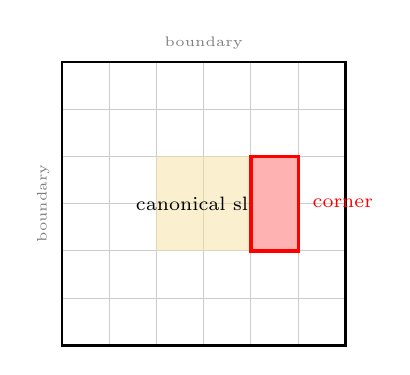
\begin{tikzpicture}[scale=0.6,font=\small]
% Matrix sketch
\draw[step=1,gray!40] (0,0) grid (6,6);
\draw[thick] (0,0) rectangle (6,6);
% A canonical slab
\fill[slab4,opacity=0.5] (2,2) rectangle (4,4);
\node[font=\scriptsize] at (3,3) {canonical slab};
% Corner witness
\fill[red!30] (4,3) rectangle (5,4);
\fill[red!30] (4,2) rectangle (5,3);
\draw[red,very thick] (4,2) rectangle (5,4);
\node[red,font=\scriptsize,right] at (5.1,3) {corner};
% Boundary labels
\node[gray,font=\tiny,rotate=90] at (-0.4,3) {boundary};
\node[gray,font=\tiny] at (3,6.4) {boundary};
\end{tikzpicture}
\end{frame}

%% ============== BACKUP 16: Rebuilding K in detail ==============
\begin{frame}{Backup: rebuilding $\mathcal{K}$ from $\mathcal{P}$ and $\mathcal{Q}$ in detail}

{\small Steps:}
\begin{enumerate}
\item Sort $\mathcal{Q}$ lexicographically in $\Oh(|\mathcal{Q}|)$ time
\item Assign 0-updates to slabs of $\mathcal{P}$ that contain them
\item For each affected slab $P=(a,b,c,d)$, process row batches $L_i$ of 0-updates with the same first coordinate
\item For each non-empty batch $L_i$: add $P[{<}i]$, split single-row slab $P[i]$ at sorted second coordinates from $L_i$, continue with $P[{>}i]$
\item Add $1\times 1$ slabs for uncovered 1-updates
\item Obtain $|\mathcal{K}|\leq |\mathcal{P}|+2|\mathcal{Q}|$, then run $\mathtt{Decompose}(n,\mathcal{K})$
\end{enumerate}

\smallskip
{\small Amortized over $8f_d(n+2)$ updates: $\Oh(\log\log n)$ per update.}

\bigskip
\centering
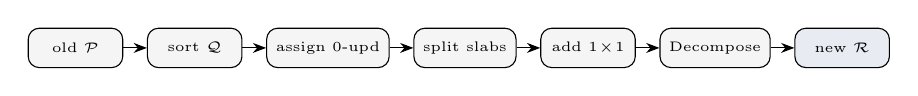
\begin{tikzpicture}[node distance=0.3cm,font=\tiny,
  box/.style={draw,rounded corners,minimum height=0.5cm,minimum width=1.2cm,fill=gray!8}]
\node[box] (p) {old $\mathcal{P}$};
\node[box,right=of p] (s) {sort $\mathcal{Q}$};
\node[box,right=of s] (a) {assign 0-upd};
\node[box,right=of a] (sp) {split slabs};
\node[box,right=of sp] (ad) {add $1\!\times\!1$};
\node[box,right=of ad] (dc) {Decompose};
\node[box,right=of dc,fill=darkblue!10] (nc) {new $\mathcal{R}$};
\draw[-{Stealth}] (p)--(s);
\draw[-{Stealth}] (s)--(a);
\draw[-{Stealth}] (a)--(sp);
\draw[-{Stealth}] (sp)--(ad);
\draw[-{Stealth}] (ad)--(dc);
\draw[-{Stealth}] (dc)--(nc);
\end{tikzpicture}

\medskip
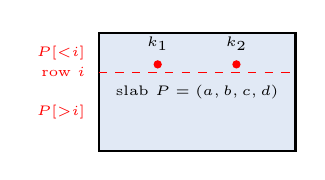
\begin{tikzpicture}[scale=0.5,font=\tiny]
% One slab being split
\fill[slab2!40] (0,0) rectangle (5,3);
\draw[thick] (0,0) rectangle (5,3);
\node at (2.5,1.5) {slab $P=(a,b,c,d)$};
% Row i
\draw[dashed,red] (0,2)--(5,2);
\node[left,red] at (-0.1,2.5) {$P[{<}i]$};
\node[left,red] at (-0.1,2) {row $i$};
\node[left,red] at (-0.1,1) {$P[{>}i]$};
% Split points in row i
\fill[red] (1.5,2.2) circle (3pt);
\fill[red] (3.5,2.2) circle (3pt);
\node[above] at (1.5,2.3) {$k_1$};
\node[above] at (3.5,2.3) {$k_2$};
\end{tikzpicture}
\end{frame}

\end{document}
